Los criterios a evaluar fueron estimados con el rango de notas de 1 a 7, sacando un promedio de cada integrante del equipo según la percepción que obtuvo al utilizar el software: \\

\begin{center}
\begin{tabular}{|l|c|p{2.40in}|}
 \hline
 \textbf{Criterio} & \textbf{Nota} & \textbf{Comentario} \\
 \hline
 \textbf{Fácil de Implementar} & 7.0 & Es una herramienta 100\% web, por lo que no necesariamente el software necesita ser instalado en el computador. \\
 \hline
 \textbf{Facilidad de uso} & 5.0 & Presenta una interfaz poco intuitiva (Diseño Drag and Drop). \\
 \hline
 \textbf{Estándares} & 6.0 & No utiliza la misma notación de BPMN 2.0 pero son semejantes, su notación esta orientada a SOA (arquitectura orientada a servicios). \\
 \hline
 \textbf{Licencia} & 7.0 & ProcessMaker brinda a las organizaciones las ventajas de open source. \\
 \hline
 \textbf{Documentación y Soporte} & 7.0 & La página web del software presenta una gran variedad de documentación , vídeos y foros en que se enseña a utilizar el software, además posee un servicio de soporte. \\
 \hline
\end{tabular}
\end{center}

\begin{center}
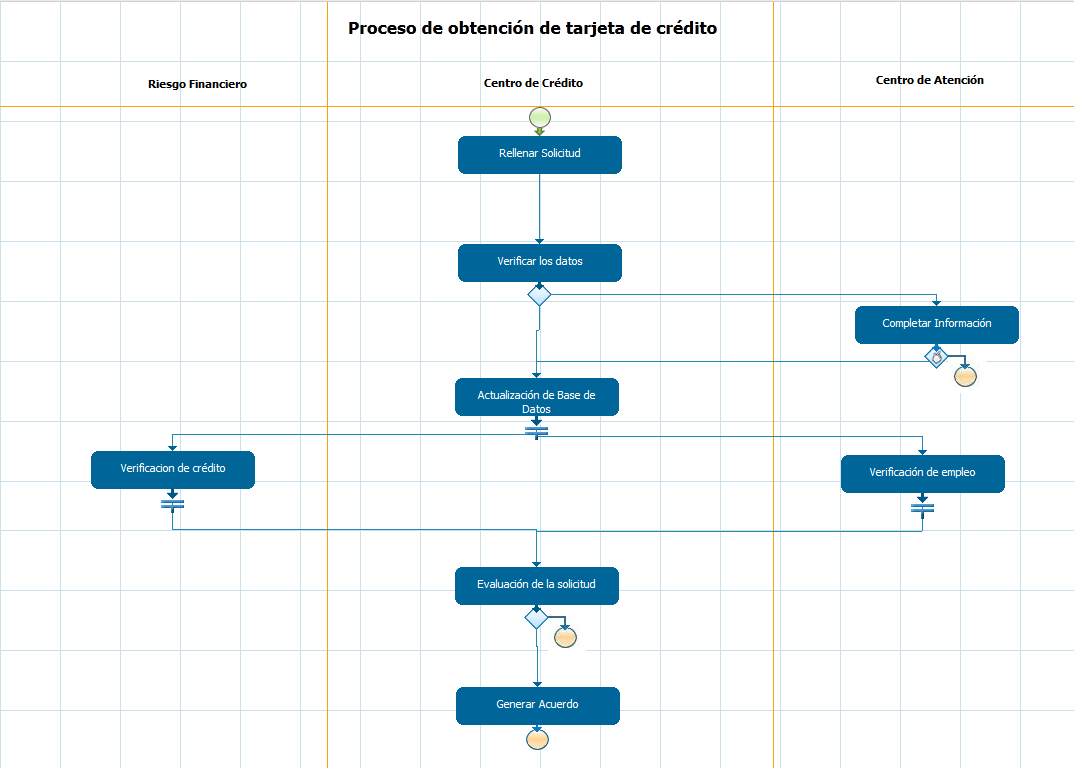
\includegraphics[scale=0.5]{./imagenes/modelos_pm.png}\\
     Figura 1: Modelo en Process Maker.\\
\end{center}